\subsection{system architecture}
% fig
\begin{figure}[t]
\begin{center}
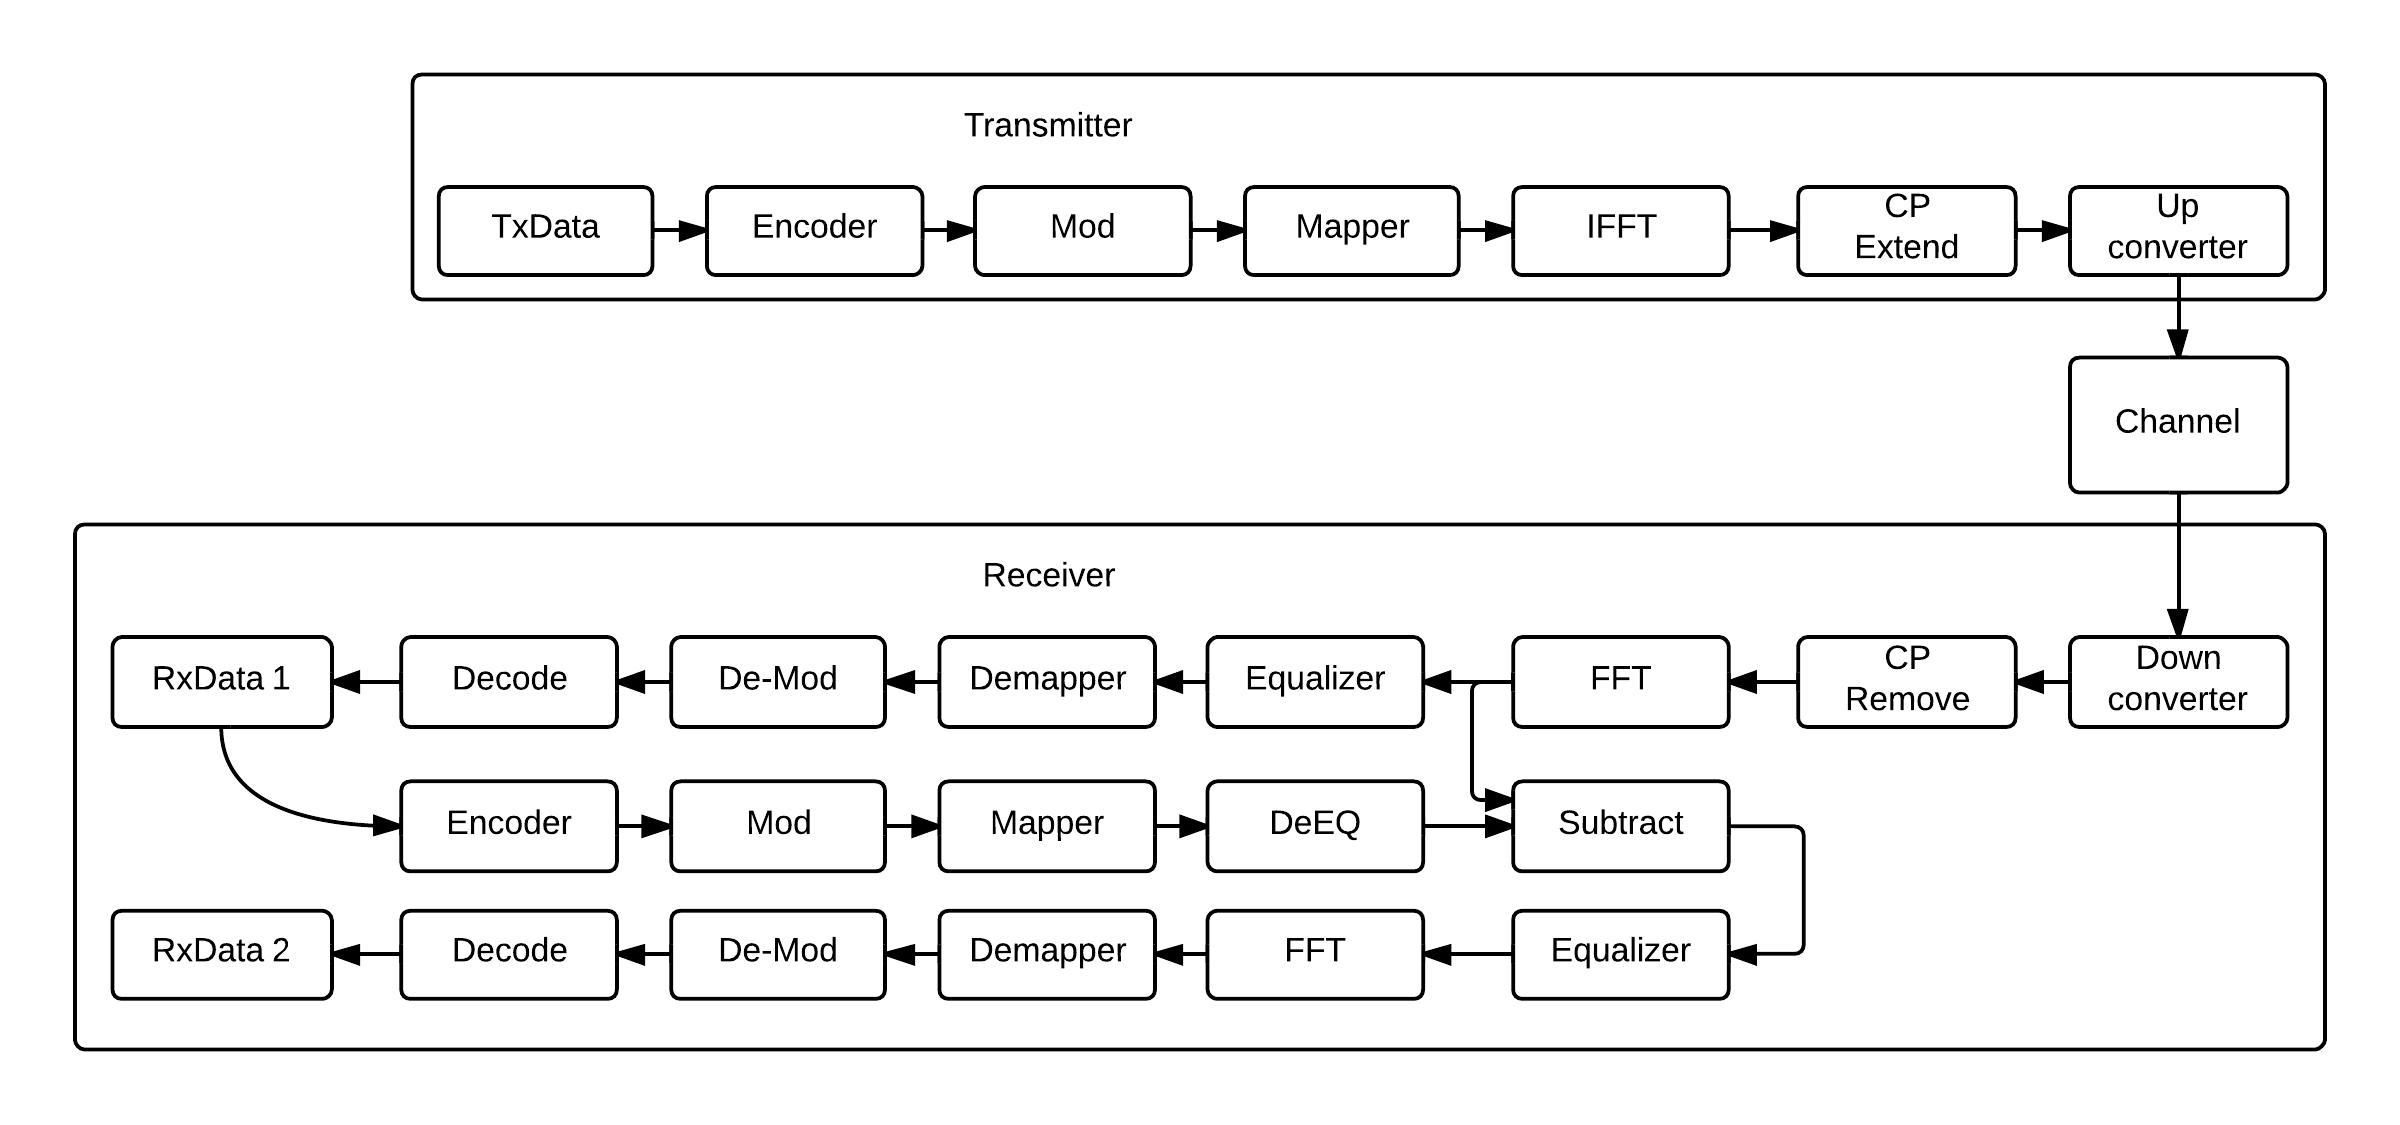
\includegraphics[width=0.95\columnwidth ,angle=0]{figure/systemArch.png}
\caption{Simulation system architecture block diagram}
\label{fig_sys_arch}
\end{center}
\end{figure}
The system architecture is shown in Fig.~\ref{fig_sys_arch}.
In this system, the receiver can only extract two layer of multiplexed data.
The values of the parameters for related blocks are listed below.
\begin{itemize}
  \item FFT size : $2048$
  \item Cyclic prefix length : $144$ samples
  \item Carrier frequency : $2.6$ GHz
  \item Bandwidth : 20MHz
  \item Modulation : BPSK, QPSK, 16QAM
  \item Coding rates : 1/2
  \item Channel : AWGN, multipath fading channel
  \item Path loss model: Hata, medium sized city
  \item Equalizer : MMSE
\end{itemize}